\paragraph{}
It is possible to add address the glaring issues in the existing system such as lack of HTTPS and an authentication mechanism.
The subsection \hyperref[subsubsec:minor-issues]{\emph{Minor Issues}} contains information around some subjects that are good to know for general security practices.
I am by no means an absolute security professional, but I do apply the measures on my own systems.

\subsection{Current Issues}\label{subsec:current-issue}
For brevity the issues are not explained in depth but that does not mean they are not insignificant.
The non-minor issues must unquestionably be addressed before large scale adoption of the current application.

\subsubsection{HTTP Connection}
\paragraph{}
It is essentially mandatory these days to use HTTPS over HTTP and in reality there is no argument to dispute this fact.
Not using HTTPS means that all traffic between the server and client is unencrypted thus being clear text.
This means any data including confidential data like user logins can be intercepted and easily read by anyone.

\subsubsection{No Authentication}
\paragraph{}
There is no authentication mechanism outside a username in each query thus making a password completely redundant.

\paragraph{Query Parameter usage}
\paragraph{}
Once you have found out that query parameters manage state and authentication impersonation becomes trivial.
\begin{description}
    \item \emph{User Impersonation:} By simply changing the \emph{user} parameter to another users' username you can use the application as
    if you were that person.
    \item \emph{Role Impersonation:} If you are a standard user you can change the \emph{admin} parameter to \emph{Y} and gain admin access.
\end{description}

\begin{figure}[h!]
    \begin{mdframed}
        http://service.cprelectrical.net.au/cpr/menu?\textcolor{violet}{admin=Y}\&\textcolor{purple}{user=LC1}
    \end{mdframed}
    \caption{Query parameters in current url}
    \label{fig:query-parameters-current}
\end{figure}

\paragraph{}
There is also the possible for accidental abuse.
For example what if a colleague wants to share a job a with someone the easiest way would be to send a link.
This link however would contain the encoded user session thus any activity from someone who launched the website from
the link would be impersonating the original user and role.

\paragraph{No Session}
\paragraph{}
Browsers have multiple ways to store key-value pairs which enables values to be stored in order to track a users authenticated status and share
secrets that only a single user/session would know. (Cookies are a good example)
The current website does not leverage any of this and thus there is no real way to identify a user outside the current URL they are using and as discussed
above this in inherently insecure.

\paragraph{}
There would be no way to "sign out" on particular devices as for all intents and purposes there us no such thing as a logged in state.


\subsubsection{Minor Issues}\label{subsubsec:minor-issues}
From a brief look at the current system I have found a few things that I mandate across my servers and would recommend for any internet
connect web server.

\paragraph{SSH Password Authentication}
It is a good practice to disable password authentication for remote SSH connections as it addresses multiple issues.
\begin{description}
    \item \emph{Brute force attacks:} Using SSH keys with a larger key-size severely reduces the viability of brute force attacks.
    \item \emph{Man in the middle attacks:} A password must be sent to the server with the potential of being intercepted by a third party.
    It is important to note that this would be highly unlikely but a risk nonetheless.
\end{description}

\paragraph{Potentially Exposed Services}
There are services like ftp and telnet listening on ports behind a firewall.
If they are not used I would turn them off and close the port entirely.
SSH is also capable of replacing these services in some scenarios.
This should be taken with a grain of salt as I don't know the internal network nor
am I a network administrator, I just thought it might be worth a mention in-case it was unintentional.



\pagebreak
\subsection{Proposed Solution}\label{subsec:proposed-solution}
It is possible to secure the current application and add authentication.
The changes would include extra development, configuration and programs to reach a suitable level of security whilst maintaining performance.
It is important to note that development time estimates and goals are only an estimate until I get to see the application hands on to get a fully
formed picture of the scope of the project.

\subsubsection{HTTPS Implementation}
HTTPS encrypts the communication channel between a client and the server preventing anyone that is listening to the line to obtain meaning data.
HTTPS implementation is next to trivial and cost free with automated tools such as \href{https://certbot.eff.org/}{\textbf{Certbot}} and 
\href{https://letsencrypt.org/}{\textbf{LetsEncrypt}}.
This automated and free implementation enables not only a set and forget mindset but also the use of shorter lease certificates to cover for
a potential certificate theft.

\paragraph{}
The current version of Apache httpd running on the server is capable of serving HTTPS traffic using TLS 1.2 and TLS 1.3 which are the current
standard at the time of writing.

\paragraph{}
In fact, I have noticed that CPR's main website is using \emph{LetsEncrypt} and short leased certificates to enable HTTPS.

\subsubsection{Token Based Authentication}
\paragraph{Replacing Query String Parameters}
The current Query String Parameters will need to be replaced for handling authentication and user sessions. 
This would take the form of access tokens that are generated on a successful login, given a short expiry then stored in an in-memory database and
send the client.

\paragraph{Unique}
This generated access token would be unique for each login enabling a multitude of security features some of which are;
\begin{description}

    \item \emph{No Stored Credentials} The client does not have their password stored in memory to add to every request,
    instead the password is only sent to gain the token before it is securely stored as a cookie.
    \item \emph{Traceability and Revocability} Access tokens can be instantly revoked when suspicious activity has been detected or an account is disabled.
    \item \emph{Generic URLS} By removing the user specific parameters from the urls they can be the exact same for all users.
    They can be shared and there is nothing to worry about when they are logged in the clients history or server connection logs.

\end{description}

\paragraph{Secure Cookie}
The access token is stored by the user as a cookie with 2 critical flags; Secure and HTTP only.
The secure flag ensure that the cookie is only sent via HTTPS traffic and the HTTP only flag restricts client side code from seeing the cookie.
Not being able to see the cookie protects the cookie from being leaked by foreign code running on the users device.

\paragraph{}
Adding Token Based Authentication will require the most development work out of the issues as code will need to be re-written and extended.
It would also be a great time to implement an in-memory database to handle tokens and user sessions without needing to do slow IO calls to a 
SQL database.

\paragraph{JWT's}
JSON Web Tokens offer a stateless form of access tokens and are often used for access tokens and session management.
There has been a conscious decision to not use JWT's as the benefits gained are not worth the loss of revocability in the case of this application.

\begin{figure}[h!]
    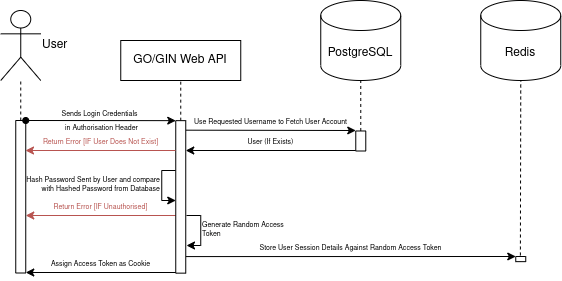
\includegraphics[width=\textwidth]{res/token_authorisation}
    \caption{A sample login process}
    \label{fig:loggin-in-sample}
\end{figure}

\subsubsection{SSH Key Authentication}
SSH implementations such as OpenSSH natively support key based authentication using asymmetric keys.
Learn more about key based authentication by reading \href{https://www.okta.com/identity-101/asymmetric-encryption/}{\textbf{this Okta article.}}
A quick synopsis is that secrets are not distributed across the network unlike password authentication.

\paragraph{}
On a Linux server that is running OpenSSH this will take no longer than 5 minutes.
However, if there are people that currently log into the system they will need to be notified and their public key uploaded to the server.

\subsection{Extra Reading}\label{subsec:extra-reading}
I have just included a few links to easy reading for a slightly more elaborate explanation on some subjects.

\begin{description}
    \item \href{https://www.cloudflare.com/en-au/learning/ssl/why-is-http-not-secure/}{\textbf{Why is HTTP Not Secure}}
    \item \href{https://wiki.archlinux.org/title/SSH_keys}{\textbf{SSH Keys}}
    \item \href{https://www.okta.com/identity-101/what-is-token-based-authentication/}{\textbf{Token Based Authentication}}
\end{description}
